% Options for packages loaded elsewhere
\PassOptionsToPackage{unicode}{hyperref}
\PassOptionsToPackage{hyphens}{url}
\documentclass[
]{article}
\usepackage{xcolor}
\usepackage[margin=1in]{geometry}
\usepackage{amsmath,amssymb}
\setcounter{secnumdepth}{-\maxdimen} % remove section numbering
\usepackage{iftex}
\ifPDFTeX
  \usepackage[T1]{fontenc}
  \usepackage[utf8]{inputenc}
  \usepackage{textcomp} % provide euro and other symbols
\else % if luatex or xetex
  \usepackage{unicode-math} % this also loads fontspec
  \defaultfontfeatures{Scale=MatchLowercase}
  \defaultfontfeatures[\rmfamily]{Ligatures=TeX,Scale=1}
\fi
\usepackage{lmodern}
\ifPDFTeX\else
  % xetex/luatex font selection
\fi
% Use upquote if available, for straight quotes in verbatim environments
\IfFileExists{upquote.sty}{\usepackage{upquote}}{}
\IfFileExists{microtype.sty}{% use microtype if available
  \usepackage[]{microtype}
  \UseMicrotypeSet[protrusion]{basicmath} % disable protrusion for tt fonts
}{}
\makeatletter
\@ifundefined{KOMAClassName}{% if non-KOMA class
  \IfFileExists{parskip.sty}{%
    \usepackage{parskip}
  }{% else
    \setlength{\parindent}{0pt}
    \setlength{\parskip}{6pt plus 2pt minus 1pt}}
}{% if KOMA class
  \KOMAoptions{parskip=half}}
\makeatother
\usepackage{longtable,booktabs,array}
\newcounter{none} % for unnumbered tables
\usepackage{calc} % for calculating minipage widths
% Correct order of tables after \paragraph or \subparagraph
\usepackage{etoolbox}
\makeatletter
\patchcmd\longtable{\par}{\if@noskipsec\mbox{}\fi\par}{}{}
\makeatother
% Allow footnotes in longtable head/foot
\IfFileExists{footnotehyper.sty}{\usepackage{footnotehyper}}{\usepackage{footnote}}
\makesavenoteenv{longtable}
\usepackage{graphicx}
\makeatletter
\newsavebox\pandoc@box
\newcommand*\pandocbounded[1]{% scales image to fit in text height/width
  \sbox\pandoc@box{#1}%
  \Gscale@div\@tempa{\textheight}{\dimexpr\ht\pandoc@box+\dp\pandoc@box\relax}%
  \Gscale@div\@tempb{\linewidth}{\wd\pandoc@box}%
  \ifdim\@tempb\p@<\@tempa\p@\let\@tempa\@tempb\fi% select the smaller of both
  \ifdim\@tempa\p@<\p@\scalebox{\@tempa}{\usebox\pandoc@box}%
  \else\usebox{\pandoc@box}%
  \fi%
}
% Set default figure placement to htbp
\def\fps@figure{htbp}
\makeatother
\setlength{\emergencystretch}{3em} % prevent overfull lines
\providecommand{\tightlist}{%
  \setlength{\itemsep}{0pt}\setlength{\parskip}{0pt}}
\usepackage{bookmark}
\IfFileExists{xurl.sty}{\usepackage{xurl}}{} % add URL line breaks if available
\urlstyle{same}
\hypersetup{
  hidelinks,
  pdfcreator={LaTeX via pandoc}}

\author{}
\date{\vspace{-2.5em}}

\begin{document}

\begin{figure}
\centering
\pandocbounded{
\includegraphics[keepaspectratio,alt={Logo UIMM}]{logo_uimm_placeholder.jpg}}
\caption{Logo UIMM}
\end{figure}

\textbf{Pôle Formation UIMM - CVDL}

\begin{center}\rule{0.5\linewidth}{0.5pt}\end{center}

\section{Atelier Cocotte LEAN, « Le Contrat Cadencé
»}\label{atelier-cocotte-lean-le-contrat-cadencuxe9}

\subsection{Guide Formateur, version
2.0}\label{guide-formateur-version-2.0}

\begin{quote}
{[}!IMPORTANT{]} \textbf{Ce que cette version change.} La v1 mesurait le
Lead Time par la loi de Little, à partir d'un WIP compté à la volée. Le
calcul ne tenait pas : la loi de Little suppose un régime permanent, or
un round de 20 minutes en flux poussé n'atteint jamais ce régime. La v2
mesure les trois indicateurs séparément et n'utilise la loi de Little
qu'en fin de journée, comme test de cohérence. C'est plus rigoureux, et
c'est devenu un temps fort du débriefing.
\end{quote}

\begin{center}\rule{0.5\linewidth}{0.5pt}\end{center}

\subsection{1. Pourquoi la version 1
échouait}\label{pourquoi-la-version-1-uxe9chouait}

Un point d'arithmétique avant tout le reste, parce qu'il explique
l'essentiel des séances ratées.

La v1 utilisait 5 postes de temps de cycle 25, 35, 40, 20 et 30
secondes, soit 150 secondes de contenu travail, avec des transferts par
lots de 10 et un round de 20 minutes.

En flux poussé par lots, la première pièce ne peut sortir du dernier
poste qu'après que chaque poste ait traité son lot complet :

\[
10 \times 25 + 10 \times 35 + 10 \times 40 + 10 \times 20 + 10 \times 30 = 1\,500\ \text{s} = 25\ \text{min}
\]

\textbf{Le round durait 20 minutes. Aucune cocotte ne sortait.}
Production nulle, taux de qualité indéfini, Lead Time non mesurable.
L'atelier ne pouvait produire aucune donnée exploitable, quelle que soit
l'énergie mise par le groupe.

Trois autres incohérences accompagnaient celle-là :

{\def\LTcaptype{none} % do not increment counter
\begin{longtable}[]{@{}
  >{\raggedright\arraybackslash}p{(\linewidth - 2\tabcolsep) * \real{0.6400}}
  >{\raggedright\arraybackslash}p{(\linewidth - 2\tabcolsep) * \real{0.3600}}@{}}
\toprule\noalign{}
\begin{minipage}[b]{\linewidth}\raggedright
Affirmation v1
\end{minipage} & \begin{minipage}[b]{\linewidth}\raggedright
Réalité
\end{minipage} \\
\midrule\noalign{}
\endhead
\bottomrule\noalign{}
\endlastfoot
Round 1 : 45 cocottes, débit 2,3 /min & Le goulot à 40 s plafonne le
débit à 1,5 /min \\
Round 3 : débit 3,4 /min & Exigerait un goulot à 17,6 s sur 5 postes \\
Takt Time de 36 s & Inférieur au goulot de 40 s : demande inatteignable
avant même le Kaizen \\
\end{longtable}
}

La v2 repose sur un modèle vérifié par simulation à événements discrets,
avec variabilité opératoire et taux de rebut. Les valeurs attendues
données dans ce guide en sont issues.

\begin{quote}
{[}!NOTE{]} \textbf{Statut des chiffres.} Les valeurs « attendues » de
ce document sont des résultats de simulation, moyennés sur 200
réplications avec une variabilité de 12 à 18 \% sur les temps
opératoires. Ce ne sont pas des relevés terrain. Elles servent au
formateur à savoir si sa séance dérive, pas à être annoncées comme
vérité aux participants.
\end{quote}

\begin{center}\rule{0.5\linewidth}{0.5pt}\end{center}

\subsection{2. Le scénario}\label{le-scuxe9nario}

\subsubsection{2.1 Le contrat}\label{le-contrat}

L'atelier est présenté comme un sous-traitant de rang 2 qui vient de
décrocher un contrat cadencé. Le formateur incarne le donneur d'ordre au
premier round, puis délègue ce rôle à un participant.

Les termes du contrat sont affichés au mur pendant toute la journée :

{\def\LTcaptype{none} % do not increment counter
\begin{longtable}[]{@{}
  >{\raggedright\arraybackslash}p{(\linewidth - 2\tabcolsep) * \real{0.5000}}
  >{\raggedright\arraybackslash}p{(\linewidth - 2\tabcolsep) * \real{0.5000}}@{}}
\toprule\noalign{}
\begin{minipage}[b]{\linewidth}\raggedright
Clause
\end{minipage} & \begin{minipage}[b]{\linewidth}\raggedright
Valeur
\end{minipage} \\
\midrule\noalign{}
\endhead
\bottomrule\noalign{}
\endlastfoot
\textbf{Volume par vacation} & 24 pièces conformes \\
\textbf{Durée de la vacation} & 16 minutes \\
\textbf{Enlèvements} & 1 camion toutes les 4 minutes, 6 pièces par
camion \\
\textbf{Qualité} & Zéro défaut accepté, tri à la charge du
fournisseur \\
\textbf{Retard} & Toute pièce manquante à l'enlèvement est reportée et
reste due \\
\end{longtable}
}

Le \textbf{Takt Time} découle directement du contrat :

\[
\text{Takt Time} = \frac{\text{Temps disponible}}{\text{Demande client}} = \frac{16 \times 60}{24} = 40\ \text{s/pièce}
\]

\subsubsection{2.2 Pourquoi ce dispositif
fonctionne}\label{pourquoi-ce-dispositif-fonctionne}

Le camion transforme le takt time en événement physique. Un participant
ne retient pas une division, il retient un carton vide qui part sans
lui. Au round 1, les deux premiers camions partent à vide et le
troisième repart à moitié plein. Personne ne conteste ensuite l'intérêt
du flux tiré.

Le rôle de client, joué par un participant, produit le second effet :
quelqu'un refuse physiquement les pièces non conformes, devant tout le
monde. Le taux de qualité cesse d'être une case à remplir.

\begin{center}\rule{0.5\linewidth}{0.5pt}\end{center}

\subsection{3. Le protocole de mesure}\label{le-protocole-de-mesure}

C'est le cœur de la refonte. Trois problèmes de la v1 sont traités par
un seul objet : le jeton.

\subsubsection{3.1 Le jeton suiveur}\label{le-jeton-suiveur}

Chaque pièce lancée en production reçoit un \textbf{jeton numéroté}
(carton plastifié, numéros 1 à 60), fixé par un trombone et qui voyage
avec elle jusqu'à la sortie.

Le jeton résout trois choses à la fois :

{\def\LTcaptype{none} % do not increment counter
\begin{longtable}[]{@{}
  >{\raggedright\arraybackslash}p{(\linewidth - 2\tabcolsep) * \real{0.3421}}
  >{\raggedright\arraybackslash}p{(\linewidth - 2\tabcolsep) * \real{0.6579}}@{}}
\toprule\noalign{}
\begin{minipage}[b]{\linewidth}\raggedright
Problème v1
\end{minipage} & \begin{minipage}[b]{\linewidth}\raggedright
Ce que le jeton apporte
\end{minipage} \\
\midrule\noalign{}
\endhead
\bottomrule\noalign{}
\endlastfoot
Lead Time calculé indirectement, résultat aberrant & Mesure directe :
heure d'entrée et heure de sortie relevées sur registre \\
En-cours difficiles à faire apparaître & WIP = nombre de jetons absents
du tableau, lisible en une seconde \\
Kanban abstrait au round 2 & Limiter le nombre de jetons plafonne
physiquement le WIP (mécanisme \textbf{CONWIP}) \\
\end{longtable}
}

\begin{quote}
{[}!TIP{]} \textbf{Le tableau des jetons} est un simple panneau A3 avec
60 emplacements numérotés. Un jeton sur le panneau signifie une place
libre dans le système. Un emplacement vide signifie une pièce en cours
quelque part sur la ligne. En un coup d'œil, sans compter, le groupe
voit le WIP monter au round 1 et rester plat au round 2.
\end{quote}

\subsubsection{3.2 Les deux registres}\label{les-deux-registres}

\textbf{Registre de lancement}, tenu par le Lanceur : numéro de jeton,
heure de lancement en mm:ss.

\textbf{Registre d'expédition}, tenu par le Client : numéro de jeton,
heure de sortie, conforme oui ou non, motif de rejet.

La base de temps est un \textbf{chronomètre projeté au mur} en mm:ss,
démarré au top départ et visible depuis tous les postes. Un chronomètre
de smartphone affiché au vidéoprojecteur suffit.

Le Lead Time de chaque pièce s'obtient par simple soustraction. On
dispose ainsi d'une distribution complète, pas d'une moyenne devinée.

\subsubsection{3.3 Les zones d'en-cours}\label{les-zones-den-cours}

Entre chaque poste, une feuille A3 posée sur la table, marquée
\textbf{ZONE D'EN-COURS P1 → P2}, et ainsi de suite. Règle absolue : une
pièce en attente est dans la zone, jamais ailleurs.

Cette contrainte matérielle est ce qui rend les stocks visibles. Sans
elle, les piles se dispersent et l'effet visuel disparaît. C'est le
point que la v1 ratait.

Au signal STOP, chaque zone est comptée séparément. Le profil d'en-cours
poste par poste désigne le goulot sans aucun calcul.

\subsubsection{3.4 Ce que chaque indicateur mesure, et
comment}\label{ce-que-chaque-indicateur-mesure-et-comment}

{\def\LTcaptype{none} % do not increment counter
\begin{longtable}[]{@{}
  >{\raggedright\arraybackslash}p{(\linewidth - 4\tabcolsep) * \real{0.3750}}
  >{\raggedright\arraybackslash}p{(\linewidth - 4\tabcolsep) * \real{0.2500}}
  >{\raggedright\arraybackslash}p{(\linewidth - 4\tabcolsep) * \real{0.3750}}@{}}
\toprule\noalign{}
\begin{minipage}[b]{\linewidth}\raggedright
Indicateur
\end{minipage} & \begin{minipage}[b]{\linewidth}\raggedright
Source
\end{minipage} & \begin{minipage}[b]{\linewidth}\raggedright
Qui relève
\end{minipage} \\
\midrule\noalign{}
\endhead
\bottomrule\noalign{}
\endlastfoot
\textbf{Takt Time} & Imposé par le contrat, non mesuré & Formateur,
affiché \\
\textbf{Temps de cycle par poste} & Chronométrage de 5 cycles
consécutifs, on retient la \textbf{médiane} & Chronométreur \\
\textbf{Temps de cycle de la ligne} & Durée du round divisée par le
nombre de pièces sorties & Client \\
\textbf{Lead Time} & Heure de sortie moins heure d'entrée, par pièce &
Calculé après coup \\
\textbf{WIP} & Comptage par zone au signal STOP & Observateur \\
\textbf{Débit} & Pièces sorties divisées par la durée & Calculé \\
\textbf{Taux de service} & Pièces livrées à l'heure sur pièces dues &
Client \\
\end{longtable}
}

\begin{quote}
{[}!NOTE{]} \textbf{Médiane et non moyenne} pour les temps de cycle. Sur
5 relevés, un incident unique (chute de ciseaux, question posée au
voisin) déforme la moyenne de 20 à 30 \%. La médiane l'ignore. C'est
aussi un point de méthode qui parle à un public industriel habitué aux
relevés de production.
\end{quote}

\begin{center}\rule{0.5\linewidth}{0.5pt}\end{center}

\subsection{4. Organisation et rôles}\label{organisation-et-ruxf4les}

\subsubsection{4.1 Une seule ligne, de 6 à 8
participants}\label{une-seule-ligne-de-6-uxe0-8-participants}

{\def\LTcaptype{none} % do not increment counter
\begin{longtable}[]{@{}
  >{\raggedright\arraybackslash}p{(\linewidth - 4\tabcolsep) * \real{0.2400}}
  >{\centering\arraybackslash}p{(\linewidth - 4\tabcolsep) * \real{0.4000}}
  >{\raggedright\arraybackslash}p{(\linewidth - 4\tabcolsep) * \real{0.3600}}@{}}
\toprule\noalign{}
\begin{minipage}[b]{\linewidth}\raggedright
Rôle
\end{minipage} & \begin{minipage}[b]{\linewidth}\centering
Effectif
\end{minipage} & \begin{minipage}[b]{\linewidth}\raggedright
Mission
\end{minipage} \\
\midrule\noalign{}
\endhead
\bottomrule\noalign{}
\endlastfoot
\textbf{Opérateur P1 à P4} & 4 & Production \\
\textbf{Lanceur} & 1 & Attribue les jetons, tient le registre de
lancement, gère le stock matière \\
\textbf{Client / Expéditeur} & 1 & Contrôle final, tient le registre
d'expédition, charge les camions, refuse les non-conformes \\
\textbf{Chronométreur} & 0 ou 1 & Relève les temps de cycle poste par
poste \\
\textbf{Observateur} & 0 ou 1 & Compte les en-cours par zone, remplit la
grille d'observation des comportements \\
\end{longtable}
}

À 6 participants, le formateur assure chronométrage et observation. À 7,
il ne garde que l'observation. À 8, il est libre d'observer le groupe,
ce qui est préférable.

\subsubsection{4.2 Rotation entre les
rounds}\label{rotation-entre-les-rounds}

Les rôles non productifs tournent entre les rounds. Les opérateurs
restent à leur poste.

C'est un arbitrage assumé : faire tourner les opérateurs remettrait à
zéro la courbe d'apprentissage et les gains du round 3 deviendraient
ininterprétables. On perd en équité de vécu, on gagne en lisibilité des
données. Annoncer cet arbitrage au groupe, sinon il est perçu comme un
oubli.

\subsubsection{4.3 Les postes}\label{les-postes}

Le carré n'est pas fourni découpé. Le poste 1 fait le débit matière, ce
qui maintient l'étape la plus génératrice de rebuts dans le périmètre et
ouvre la principale piste Kaizen.

{\def\LTcaptype{none} % do not increment counter
\begin{longtable}[]{@{}
  >{\centering\arraybackslash}p{(\linewidth - 4\tabcolsep) * \real{0.1458}}
  >{\raggedright\arraybackslash}p{(\linewidth - 4\tabcolsep) * \real{0.2500}}
  >{\centering\arraybackslash}p{(\linewidth - 4\tabcolsep) * \real{0.6042}}@{}}
\toprule\noalign{}
\begin{minipage}[b]{\linewidth}\centering
Poste
\end{minipage} & \begin{minipage}[b]{\linewidth}\raggedright
Opérations
\end{minipage} & \begin{minipage}[b]{\linewidth}\centering
Temps de cycle de référence
\end{minipage} \\
\midrule\noalign{}
\endhead
\bottomrule\noalign{}
\endlastfoot
\textbf{P1} & Débit matière : triangle, découpe de la chute, carré 210 ×
210 & 25 s \\
\textbf{P2} & Diagonales puis premier blintz, 4 coins au centre & 30
s \\
\textbf{P3} & Retournement puis second blintz, 4 coins au centre & 35
s \\
\textbf{P4} & Pré-formage, mise en volume & 25 s \\
& \textbf{Contenu travail total} & \textbf{115 s} \\
\end{longtable}
}

\textbf{Goulot initial : P3 à 35 secondes.} Débit maximal théorique de
la ligne : 1,71 pièce par minute, soit 27 pièces sur une vacation de 16
minutes. La demande de 24 pièces est donc atteignable, mais seulement si
le système ne perd rien en attente, en reprise ou en rebut. C'est la
tension qui fait tenir la journée.

\begin{center}\rule{0.5\linewidth}{0.5pt}\end{center}

\subsection{5. Standard de pliage (FIP)}\label{standard-de-pliage-fip}

\begin{quote}
\textbf{Objectif} : produire une cocotte symétrique, fonctionnelle, sans
déchirure.

\textbf{Matière} : 1 feuille A4 blanche 80 g/m².
\end{quote}

\subsubsection{5.1 Obtenir le carré}\label{obtenir-le-carruxe9}

\begin{enumerate}
\def\labelenumi{\arabic{enumi}.}
\tightlist
\item
  \textbf{Le triangle} : rabattre le coin supérieur gauche sur le bord
  droit pour former un triangle rectangle isocèle.
\item
  \textbf{La chute} : découper ou déchirer proprement le long du pli la
  bande rectangulaire restante.
\item
  \textbf{Résultat} : carré de 210 × 210 mm.
\end{enumerate}

\begin{quote}
{[}!TIP{]} La majorité des rebuts du round 1 vient d'un carré mal
équerré. Ne pas le dire au groupe avant le débriefing. C'est ce constat
qui déclenchera la proposition du gabarit au round 3.
\end{quote}

\subsubsection{5.2 Les étapes}\label{les-uxe9tapes}

{\def\LTcaptype{none} % do not increment counter
\begin{longtable}[]{@{}
  >{\centering\arraybackslash}p{(\linewidth - 6\tabcolsep) * \real{0.2059}}
  >{\raggedright\arraybackslash}p{(\linewidth - 6\tabcolsep) * \real{0.2353}}
  >{\raggedright\arraybackslash}p{(\linewidth - 6\tabcolsep) * \real{0.3235}}
  >{\raggedright\arraybackslash}p{(\linewidth - 6\tabcolsep) * \real{0.2353}}@{}}
\toprule\noalign{}
\begin{minipage}[b]{\linewidth}\centering
Étape
\end{minipage} & \begin{minipage}[b]{\linewidth}\raggedright
Action
\end{minipage} & \begin{minipage}[b]{\linewidth}\raggedright
Point clé
\end{minipage} & \begin{minipage}[b]{\linewidth}\raggedright
Raison
\end{minipage} \\
\midrule\noalign{}
\endhead
\bottomrule\noalign{}
\endlastfoot
\textbf{1} & \textbf{Les diagonales} & Marquer les deux plis en croix
coin à coin & Localiser le centre exact \\
\textbf{2} & \textbf{Premier blintz} & Rabattre les 4 coins vers le
centre & Les bords ne doivent pas se chevaucher \\
\textbf{3} & \textbf{Le retournement} & Retourner la feuille, face lisse
vers soi & Conditionne la cinématique d'ouverture \\
\textbf{4} & \textbf{Second blintz} & Rabattre les 4 nouveaux coins vers
le centre & Appuyer fort, marquer le pli \\
\textbf{5} & \textbf{Pré-formage} & Plier en deux horizontalement puis
verticalement & Marquer les plis extérieurs \\
\textbf{6} & \textbf{Mise en volume} & Glisser les doigts dans les 4
poches, pousser vers le centre & Ne pas déchirer \\
\end{longtable}
}

\begin{figure}
\centering
\pandocbounded{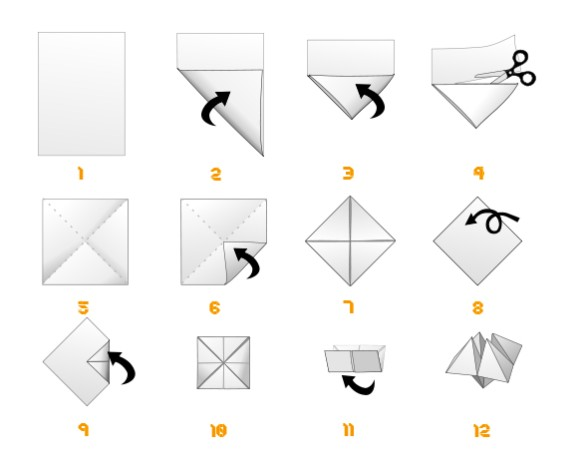
\includegraphics[keepaspectratio,alt={Plan de pliage}]{Plan_Cocotte_simple.jpg}}
\caption{Plan de pliage}
\end{figure}

\subsubsection{5.3 Critères de
conformité}\label{crituxe8res-de-conformituxe9}

{\def\LTcaptype{none} % do not increment counter
\begin{longtable}[]{@{}
  >{\centering\arraybackslash}p{(\linewidth - 4\tabcolsep) * \real{0.1364}}
  >{\raggedright\arraybackslash}p{(\linewidth - 4\tabcolsep) * \real{0.4091}}
  >{\raggedright\arraybackslash}p{(\linewidth - 4\tabcolsep) * \real{0.4545}}@{}}
\toprule\noalign{}
\begin{minipage}[b]{\linewidth}\centering
\#
\end{minipage} & \begin{minipage}[b]{\linewidth}\raggedright
Critère
\end{minipage} & \begin{minipage}[b]{\linewidth}\raggedright
Contrôle
\end{minipage} \\
\midrule\noalign{}
\endhead
\bottomrule\noalign{}
\endlastfoot
1 & \textbf{Symétrie} & Les 4 pointes à même hauteur, vérification
visuelle sur plan \\
2 & \textbf{Mobilité} & Ouverture et fermeture sans résistance, 3
actionnements dans les deux axes \\
3 & \textbf{Intégrité} & Aucune déchirure, aucun pli parasite \\
\end{longtable}
}

Le contrôle est fait par le Client, à réception. Une pièce refusée est
posée dans le \textbf{bac rouge}, comptée en rebut, et n'est jamais
recomptée.

\begin{center}\rule{0.5\linewidth}{0.5pt}\end{center}

\subsection{6. Round 1 : Flux poussé, transfert par lots de
5}\label{round-1-flux-poussuxe9-transfert-par-lots-de-5}

\subsubsection{6.1 Règles annoncées au
groupe}\label{ruxe8gles-annoncuxe9es-au-groupe}

\begin{quote}
{[}!WARNING{]} - Transfert par \textbf{lots de 5}. Un poste ne transmet
que lorsque ses 5 pièces sont finies. - Chaque poste produit \textbf{au
maximum de sa capacité}, sans jamais attendre l'aval. -
\textbf{Communication interdite} entre postes. - Objectif donné : «
produire le maximum ». - Le Lanceur dispose des \textbf{60 jetons}. Il
lance sans limite.
\end{quote}

\subsubsection{6.2 Pièges de conduite}\label{piuxe8ges-de-conduite}

\begin{quote}
{[}!CAUTION{]} \textbf{Ne pas faire circuler un seul lot à la fois.}
Tous les postes doivent tourner en parallèle dès qu'ils ont de la
matière. C'est le parallélisme qui crée l'accumulation. Si le formateur
laisse le groupe traiter un lot du début à la fin, l'effet ne se produit
pas.

\textbf{Le P1 ne s'arrête jamais.} Il a un stock matière de 60 feuilles
devant lui. C'est lui qui alimente la montagne d'en-cours. Si le P1
ralentit par empathie pour l'aval, l'expérience s'effondre. Le formateur
le relance : « votre indicateur à vous, c'est votre production ».
\end{quote}

\subsubsection{6.3 Déroulé}\label{duxe9rouluxe9}

{\def\LTcaptype{none} % do not increment counter
\begin{longtable}[]{@{}
  >{\raggedright\arraybackslash}p{(\linewidth - 2\tabcolsep) * \real{0.4118}}
  >{\raggedright\arraybackslash}p{(\linewidth - 2\tabcolsep) * \real{0.5882}}@{}}
\toprule\noalign{}
\begin{minipage}[b]{\linewidth}\raggedright
Temps
\end{minipage} & \begin{minipage}[b]{\linewidth}\raggedright
Séquence
\end{minipage} \\
\midrule\noalign{}
\endhead
\bottomrule\noalign{}
\endlastfoot
0 à 5 min & Briefing, distribution des jetons, mise en place du chrono
projeté \\
5 à 21 min & \textbf{Vacation de 16 minutes.} Le formateur circule sans
intervenir. Camions à 4, 8, 12 et 16 min \\
21 à 29 min & \textbf{STOP.} Comptage par zone, clôture des registres,
remplissage du tableau de marche \\
29 à 50 min & Débriefing \\
\end{longtable}
}

\subsubsection{6.4 Résultats attendus}\label{ruxe9sultats-attendus}

{\def\LTcaptype{none} % do not increment counter
\begin{longtable}[]{@{}lc@{}}
\toprule\noalign{}
Indicateur & Valeur attendue \\
\midrule\noalign{}
\endhead
\bottomrule\noalign{}
\endlastfoot
Pièces lancées & 38 à 42 \\
Pièces sorties & 13 à 16 \\
Pièces conformes & 10 à 12 \\
\textbf{WIP en fin de vacation} & \textbf{24 à 28} \\
\textbf{Lead Time moyen} & \textbf{environ 10 min} \\
Débit & 0,9 /min \\
Temps de cycle de la ligne & environ 66 s, pour un takt de 40 s \\
\textbf{Taux de service client} & \textbf{environ 45 \%} \\
Camions partis vides & \textbf{les deux premiers} \\
\end{longtable}
}

\subsubsection{6.5 Le chiffre qui frappe}\label{le-chiffre-qui-frappe}

\[
\text{Ratio d'efficacité du processus} = \frac{\text{Contenu travail}}{\text{Lead Time}} = \frac{115\ \text{s}}{620\ \text{s}} \approx 18\ \%
\]

Sur les dix minutes que passe une cocotte dans l'atelier, moins de deux
minutes servent à la transformer. Le reste, elle attend. Écrire ce ratio
au paperboard et le laisser affiché toute la journée.

\subsubsection{6.6 Questions de
débriefing}\label{questions-de-duxe9briefing}

Dans cet ordre, sans en sauter :

\begin{enumerate}
\def\labelenumi{\arabic{enumi}.}
\tightlist
\item
  « Qui a eu le sentiment de bien travailler ? » (presque tous lèvent la
  main, alors que le client n'a reçu que la moitié de sa commande)
\item
  « Regardez les zones d'en-cours. Où est la plus haute pile ? » (le
  groupe désigne le goulot lui-même, sans calcul)
\item
  « Combien de temps une cocotte a-t-elle passé dans l'atelier ? Combien
  de temps a-t-elle été travaillée ? »
\item
  « Quand avez-vous su qu'il y avait un défaut de découpe ? » (à la
  sortie, sur des pièces produites dix minutes plus tôt)
\item
  « Le standard était scotché sur votre table. Qui l'a lu pendant la
  vacation ? »
\item
  Identification des gaspillages observés, au paperboard, en s'appuyant
  sur ce qui vient d'être vécu et non sur la liste théorique
\end{enumerate}

\subsubsection{6.7 Gaspillages à faire
émerger}\label{gaspillages-uxe0-faire-uxe9merger}

{\def\LTcaptype{none} % do not increment counter
\begin{longtable}[]{@{}
  >{\raggedright\arraybackslash}p{(\linewidth - 2\tabcolsep) * \real{0.2609}}
  >{\raggedright\arraybackslash}p{(\linewidth - 2\tabcolsep) * \real{0.7391}}@{}}
\toprule\noalign{}
\begin{minipage}[b]{\linewidth}\raggedright
Gaspillage
\end{minipage} & \begin{minipage}[b]{\linewidth}\raggedright
Manifestation observable ce jour
\end{minipage} \\
\midrule\noalign{}
\endhead
\bottomrule\noalign{}
\endlastfoot
Surproduction & 40 pièces lancées pour 24 demandées \\
Stocks & Les zones d'en-cours saturées \\
Attentes & P4 inactif pendant les 7 premières minutes \\
Défauts & Rebuts détectés en fin de ligne, sur des pièces anciennes \\
Sur-processus & Reprises de pliage sur des carrés mal équerrés \\
Mouvements & Recherche de place pour poser les piles \\
Transports & Déplacements pour transférer les lots \\
Sous-emploi des compétences & Personne n'a le droit de parler ni de
proposer quoi que ce soit \\
\end{longtable}
}

\begin{center}\rule{0.5\linewidth}{0.5pt}\end{center}

\subsection{7. Round 2 : Flux tiré, CONWIP à 6
jetons}\label{round-2-flux-tiruxe9-conwip-uxe0-6-jetons}

\subsubsection{7.1 Apport préalable, 30
minutes}\label{apport-pruxe9alable-30-minutes}

Trois notions, dans cet ordre :

\textbf{Flux tiré.} On ne produit que sur demande de l'aval. Inversion
du sens de l'information.

\textbf{Kanban.} Le signal de production. Ici, le jeton libre remplace
la carte : pas de jeton, pas de lancement.

\textbf{CONWIP.} Plafonner le nombre de jetons en circulation revient à
plafonner le WIP. Le lien avec le Lead Time se déduit ensuite du relevé
du round 1, sans avoir besoin de la formule.

\subsubsection{7.2 Règles}\label{ruxe8gles}

\begin{quote}
{[}!TIP{]} - Transfert \textbf{pièce à pièce}. Aucun lot. - Le Lanceur
ne dispose que de \textbf{6 jetons}. Il ne peut lancer une pièce que si
un jeton est revenu. - Un poste ne prend une pièce que lorsqu'il est
libre. Une seule pièce en attente maximum entre deux postes. -
\textbf{Communication autorisée et encouragée.} Un poste qui reçoit une
pièce douteuse la renvoie immédiatement en amont. - Réimplantation
autorisée : rapprocher les tables. - Objectif donné : « livrer les 4
camions ».
\end{quote}

\subsubsection{7.3 Déroulé}\label{duxe9rouluxe9-1}

{\def\LTcaptype{none} % do not increment counter
\begin{longtable}[]{@{}
  >{\raggedright\arraybackslash}p{(\linewidth - 2\tabcolsep) * \real{0.4118}}
  >{\raggedright\arraybackslash}p{(\linewidth - 2\tabcolsep) * \real{0.5882}}@{}}
\toprule\noalign{}
\begin{minipage}[b]{\linewidth}\raggedright
Temps
\end{minipage} & \begin{minipage}[b]{\linewidth}\raggedright
Séquence
\end{minipage} \\
\midrule\noalign{}
\endhead
\bottomrule\noalign{}
\endlastfoot
0 à 8 min & Briefing, réimplantation, retrait de 54 jetons du tableau \\
8 à 12 min & Essai à blanc, 4 pièces \\
12 à 28 min & \textbf{Vacation de 16 minutes} \\
28 à 34 min & STOP, comptage, registres, tableau de marche \\
34 à 50 min & Débriefing \\
\end{longtable}
}

\subsubsection{7.4 Résultats attendus}\label{ruxe9sultats-attendus-1}

{\def\LTcaptype{none} % do not increment counter
\begin{longtable}[]{@{}lcc@{}}
\toprule\noalign{}
Indicateur & Round 1 & Round 2 attendu \\
\midrule\noalign{}
\endhead
\bottomrule\noalign{}
\endlastfoot
Pièces sorties & 13 à 16 & 23 à 26 \\
Pièces conformes & 10 à 12 & 20 à 23 \\
\textbf{WIP} & 24 à 28 & \textbf{6, par construction} \\
\textbf{Lead Time} & environ 10 min & \textbf{environ 3,5 min} \\
Débit & 0,9 /min & 1,5 /min \\
Temps de cycle ligne & 66 s & environ 39 s, takt à 40 s \\
Ratio d'efficacité & 18 \% & \textbf{environ 55 \%} \\
Taux de service & 45 \% & 80 à 100 \% \\
\end{longtable}
}

\begin{quote}
{[}!IMPORTANT{]} \textbf{Le point à ne pas manquer.} Le débit n'a pas
augmenté parce que les gens travaillent plus vite. Les temps de cycle
par poste sont les mêmes. Ce qui a changé, c'est que la ligne ne
fabrique plus ce dont personne n'a besoin. Poser la question ainsi : «
qui a travaillé plus vite ce round ? Personne. Alors d'où viennent les
10 pièces de plus ? »
\end{quote}

\subsubsection{7.5 Questions de
débriefing}\label{questions-de-duxe9briefing-1}

\begin{enumerate}
\def\labelenumi{\arabic{enumi}.}
\tightlist
\item
  « Combien de pièces avez-vous eu sous la main en même temps ? » (six,
  jamais plus, et ils l'ont senti)
\item
  « Quand avez-vous détecté les défauts cette fois ? »
\item
  « Le premier camion est-il parti plein ? » (non, la montée en charge
  existe toujours, mais le retard se rattrape au lieu de se creuser)
\item
  « Qu'est-ce qui vous a le plus gêné ? » (l'attente devant le goulot,
  ce qui ouvre le round 3)
\end{enumerate}

\begin{center}\rule{0.5\linewidth}{0.5pt}\end{center}

\subsection{8. Chantier Kaizen : 45
minutes}\label{chantier-kaizen-45-minutes}

\subsubsection{8.1 Yamazumi}\label{yamazumi}

Le chronométreur a relevé les temps de cycle des deux rounds. On
construit le diagramme au paperboard :

\begin{verbatim}
Temps (s)
  40 │                    Takt Time = 40 s
     ├ ─ ─ ─ ─ ─ ─ ─ ─ ─ ─ ─ ─ ─ ─ ─ ─ ─ ─
  35 │              ████
  30 │       ████   ████
  25 │ ████  ████   ████   ████
  20 │ ████  ████   ████   ████
  15 │ ████  ████   ████   ████
  10 │ ████  ████   ████   ████
   5 │ ████  ████   ████   ████
   0 └──┬─────┬──────┬──────┬───
        P1    P2     P3     P4
       25 s  30 s   35 s   25 s
\end{verbatim}

Aucun poste ne dépasse le takt. Le problème n'est donc pas la capacité,
c'est le \textbf{déséquilibre} : 10 secondes d'écart entre P1 et P3
signifient que P1 et P4 attendent en permanence. C'est du \textbf{Mura},
et c'est ce qui limite le débit réel.

\subsubsection{8.2 Conduite du
brainstorming}\label{conduite-du-brainstorming}

Ne pas donner les solutions. Poser la question et laisser chercher 15
minutes en équipe complète, formateur en retrait.

Solutions généralement trouvées par les groupes :

{\def\LTcaptype{none} % do not increment counter
\begin{longtable}[]{@{}
  >{\raggedright\arraybackslash}p{(\linewidth - 4\tabcolsep) * \real{0.3182}}
  >{\raggedright\arraybackslash}p{(\linewidth - 4\tabcolsep) * \real{0.3182}}
  >{\raggedright\arraybackslash}p{(\linewidth - 4\tabcolsep) * \real{0.3636}}@{}}
\toprule\noalign{}
\begin{minipage}[b]{\linewidth}\raggedright
Piste
\end{minipage} & \begin{minipage}[b]{\linewidth}\raggedright
Effet
\end{minipage} & \begin{minipage}[b]{\linewidth}\raggedright
Nature
\end{minipage} \\
\midrule\noalign{}
\endhead
\bottomrule\noalign{}
\endlastfoot
\textbf{Gabarit carton 210 × 210} au P1, on trace au lieu de mesurer &
P1 : 25 s → 20 s, et rebuts de découpe quasi éliminés & Poka-yoké \\
\textbf{Retournement transféré à P2}, qui a la pièce en main en fin
d'opération & P3 : 35 s → 30 s, coût marginal nul pour P2 &
Rééquilibrage \\
\textbf{Un coin du second blintz transféré à P4} & P3 : 30 s → 28 s, P4
: 25 s → 27 s & Rééquilibrage \\
\textbf{Pliage contre le bord d'une règle} & P2 : 30 s → 27 s, plis
mieux marqués & Standard de geste \\
\end{longtable}
}

\begin{quote}
{[}!TIP{]} Le formateur garde un gabarit carton prêt, caché. Si le
groupe ne trouve pas au bout de 10 minutes, il pose la question : «
qu'est-ce qui prend du temps dans la découpe, le geste ou la
vérification ? ». La réponse mène au gabarit sans le donner.
\end{quote}

Résultat cible après chantier :

{\def\LTcaptype{none} % do not increment counter
\begin{longtable}[]{@{}ccc@{}}
\toprule\noalign{}
Poste & Avant & Après \\
\midrule\noalign{}
\endhead
\bottomrule\noalign{}
\endlastfoot
P1 & 25 s & 20 s \\
P2 & 30 s & 27 s \\
P3 & \textbf{35 s} & 28 s \\
P4 & 25 s & 27 s \\
\textbf{Contenu travail} & 115 s & \textbf{102 s} \\
\textbf{Goulot} & 35 s & \textbf{28 s} \\
\end{longtable}
}

Le gain sur le contenu travail est de 11 \%. Le gain sur le goulot est
de 20 \%. Ne pas promettre davantage : un chantier de 45 minutes ne
produit pas de miracle, et annoncer des gains irréalistes discrédite la
méthode auprès d'un public qui connaît son atelier.

\subsubsection{8.3 Chantier 5S : 15
minutes}\label{chantier-5s-15-minutes}

{\def\LTcaptype{none} % do not increment counter
\begin{longtable}[]{@{}
  >{\centering\arraybackslash}p{(\linewidth - 4\tabcolsep) * \real{0.0833}}
  >{\raggedright\arraybackslash}p{(\linewidth - 4\tabcolsep) * \real{0.1944}}
  >{\raggedright\arraybackslash}p{(\linewidth - 4\tabcolsep) * \real{0.7222}}@{}}
\toprule\noalign{}
\begin{minipage}[b]{\linewidth}\centering
\#
\end{minipage} & \begin{minipage}[b]{\linewidth}\raggedright
Terme
\end{minipage} & \begin{minipage}[b]{\linewidth}\raggedright
Action concrète au poste
\end{minipage} \\
\midrule\noalign{}
\endhead
\bottomrule\noalign{}
\endlastfoot
1 & \textbf{Seiri} & Retirer de la table tout ce qui ne sert pas à
l'opération \\
2 & \textbf{Seiton} & Placer ciseaux, règle et gabarit dans la zone de
préhension, toujours au même endroit \\
3 & \textbf{Seiso} & Évacuer les chutes de découpe au fur et à mesure \\
4 & \textbf{Seiketsu} & Photographier le poste rangé, afficher la photo
au poste \\
5 & \textbf{Shitsuke} & Le poste est remis dans l'état de la photo à
chaque fin de vacation \\
\end{longtable}
}

\begin{center}\rule{0.5\linewidth}{0.5pt}\end{center}

\subsection{9. Round 3 : Ligne équilibrée, CONWIP à 4
jetons}\label{round-3-ligne-uxe9quilibruxe9e-conwip-uxe0-4-jetons}

\subsubsection{9.1 Règles}\label{ruxe8gles-1}

Identiques au round 2, avec les améliorations en place et \textbf{4
jetons seulement}.

Réduire encore le WIP est contre-intuitif pour le groupe : « on va
produire moins ». C'est le moment de le laisser tester et constater
l'inverse.

\subsubsection{9.2 Résultats attendus}\label{ruxe9sultats-attendus-2}

{\def\LTcaptype{none} % do not increment counter
\begin{longtable}[]{@{}lccc@{}}
\toprule\noalign{}
Indicateur & R1 & R2 & R3 attendu \\
\midrule\noalign{}
\endhead
\bottomrule\noalign{}
\endlastfoot
Pièces sorties & 13-16 & 23-26 & 28-32 \\
Pièces conformes & 10-12 & 21-23 & 28-30 \\
\textbf{WIP} & 24-28 & 6 & \textbf{4} \\
\textbf{Lead Time} & \textasciitilde10 min & \textasciitilde3,5 min &
\textbf{\textasciitilde2 min} \\
Débit & 0,9 /min & 1,5 /min & 1,9 /min \\
Temps de cycle ligne & 66 s & 39 s & 32 s \\
\textbf{Ratio d'efficacité} & 18 \% & 55 \% & \textbf{85 \%} \\
Taux de service & 45 \% & 90-100 \% & 100 \% \\
\end{longtable}
}

\subsubsection{9.3 Le piège volontaire du round
3}\label{le-piuxe8ge-volontaire-du-round-3}

La ligne équilibrée produit environ 29 pièces conformes. Le client en
demande 24.

\textbf{Les 5 pièces excédentaires sont de la surproduction.} Elles ne
sont pas vendues, elles ont consommé de la matière et du temps, elles
encombrent.

Poser la question au débriefing : « vous avez fait 29 pièces, le client
en voulait 24. C'est une bonne ou une mauvaise performance ? » Le groupe
répond spontanément « bonne ». C'est le moment d'introduire la règle du
takt : \textbf{produire au rythme du client, ni plus vite ni moins
vite.} Une ligne qui produit trop vite doit ralentir et affecter le
temps libéré à autre chose, pas fabriquer du stock.

C'est le point le plus contre-intuitif de la journée et celui qui reste
le plus longtemps.

\subsubsection{9.4 Variante pour public
confirmé}\label{variante-pour-public-confirmuxe9}

Porter la demande à 32 pièces (8 par camion, takt de 30 s) uniquement au
round 3. La ligne équilibrée en est tout juste capable, à condition de
zéro arrêt et de zéro rebut. On perd la comparabilité directe avec les
rounds précédents, on gagne une tension réaliste. À réserver aux groupes
qui ont bien tenu les rounds 1 et 2.

\begin{center}\rule{0.5\linewidth}{0.5pt}\end{center}

\subsection{10. Synthèse : 30 minutes}\label{synthuxe8se-30-minutes}

\subsubsection{10.1 Les trois indicateurs}\label{les-trois-indicateurs}

{\def\LTcaptype{none} % do not increment counter
\begin{longtable}[]{@{}
  >{\raggedright\arraybackslash}p{(\linewidth - 6\tabcolsep) * \real{0.0714}}
  >{\raggedright\arraybackslash}p{(\linewidth - 6\tabcolsep) * \real{0.2857}}
  >{\raggedright\arraybackslash}p{(\linewidth - 6\tabcolsep) * \real{0.3333}}
  >{\raggedright\arraybackslash}p{(\linewidth - 6\tabcolsep) * \real{0.3095}}@{}}
\toprule\noalign{}
\begin{minipage}[b]{\linewidth}\raggedright
\end{minipage} & \begin{minipage}[b]{\linewidth}\raggedright
Définition
\end{minipage} & \begin{minipage}[b]{\linewidth}\raggedright
Ce qu'il dit
\end{minipage} & \begin{minipage}[b]{\linewidth}\raggedright
Qui le fixe
\end{minipage} \\
\midrule\noalign{}
\endhead
\bottomrule\noalign{}
\endlastfoot
\textbf{Takt Time} & Temps disponible / demande client & À quel rythme
il \textbf{faut} produire & Le client \\
\textbf{Temps de cycle} & Temps de traitement / pièces produites & À
quel rythme on produit \textbf{réellement} & Le processus \\
\textbf{Lead Time} & Temps entre entrée matière et livraison & Combien
de temps le client \textbf{attend} & Le système entier \\
\end{longtable}
}

\[
\text{Takt Time} = \frac{\text{Temps disponible}}{\text{Demande client}}
\qquad
\text{Temps de cycle} = \frac{\text{Temps de traitement}}{\text{Nombre de pièces}}
\]

\[
\text{Lead Time} = \sum \text{Temps d'attente} + \sum \text{Temps de transport} + \sum \text{Temps de traitement}
\]

\textbf{La règle} : si le temps de cycle dépasse le takt time, la
demande ne peut pas être tenue. S'il est très inférieur, on surproduit.
On vise l'égalité.

\subsubsection{10.2 La loi de Little, en test et non en
outil}\label{la-loi-de-little-en-test-et-non-en-outil}

\[
\boxed{\text{WIP} = \text{Débit} \times \text{Lead Time}}
\]

On dispose maintenant des trois grandeurs \textbf{mesurées séparément}.
On confronte.

{\def\LTcaptype{none} % do not increment counter
\begin{longtable}[]{@{}
  >{\centering\arraybackslash}p{(\linewidth - 10\tabcolsep) * \real{0.0737}}
  >{\centering\arraybackslash}p{(\linewidth - 10\tabcolsep) * \real{0.1263}}
  >{\centering\arraybackslash}p{(\linewidth - 10\tabcolsep) * \real{0.1474}}
  >{\centering\arraybackslash}p{(\linewidth - 10\tabcolsep) * \real{0.3474}}
  >{\centering\arraybackslash}p{(\linewidth - 10\tabcolsep) * \real{0.2316}}
  >{\centering\arraybackslash}p{(\linewidth - 10\tabcolsep) * \real{0.0737}}@{}}
\toprule\noalign{}
\begin{minipage}[b]{\linewidth}\centering
Round
\end{minipage} & \begin{minipage}[b]{\linewidth}\centering
WIP mesuré
\end{minipage} & \begin{minipage}[b]{\linewidth}\centering
Débit mesuré
\end{minipage} & \begin{minipage}[b]{\linewidth}\centering
Lead Time \textbf{prédit} par Little
\end{minipage} & \begin{minipage}[b]{\linewidth}\centering
Lead Time \textbf{mesuré}
\end{minipage} & \begin{minipage}[b]{\linewidth}\centering
Écart
\end{minipage} \\
\midrule\noalign{}
\endhead
\bottomrule\noalign{}
\endlastfoot
1 & 26 & 0,90 /min & 28,9 min & 10,4 min & \textbf{facteur 2,8} \\
2 & 6 & 1,53 /min & 3,9 min & 3,5 min & 11 \% \\
3 & 4 & 1,89 /min & 2,1 min & 2,0 min & 5 \% \\
\end{longtable}
}

\begin{quote}
{[}!IMPORTANT{]} \textbf{C'est le moment intellectuel fort de la
journée.} La loi de Little est exacte, mais elle suppose un
\textbf{régime permanent} : un système dont le WIP moyen ne dérive pas.
Aux rounds 2 et 3, le CONWIP force ce régime, et la loi tombe juste à 5
\% près. Au round 1, le WIP grimpe sans arrêt pendant toute la vacation,
le système n'est jamais stationnaire, et la loi donne un résultat faux.

Traduction pour l'atelier : \textbf{une usine en flux poussé est une
usine dont on ne sait pas prédire les délais.} Ce n'est pas un problème
de formule, c'est un problème de pilotage. On ne peut pas promettre une
date de livraison à un client quand on ne maîtrise pas son propre WIP.
\end{quote}

Cette démonstration remplace avantageusement l'usage de la loi de Little
comme méthode de calcul, qui donnait des Lead Times aberrants et
décrédibilisait l'ensemble.

\subsubsection{10.3 TRG}\label{trg}

Définitions conformes à la \textbf{norme NF E 60-182} :

\[
\text{TRS} = \frac{\text{Temps utile}}{\text{Temps requis}}
\qquad
\text{TRG} = \frac{\text{Temps utile}}{\text{Temps d'ouverture}}
\qquad
\text{TRE} = \frac{\text{Temps utile}}{\text{Temps total}}
\]

Dans l'atelier, temps d'ouverture et temps requis sont confondus, il n'y
a pas d'arrêt planifié dans une vacation. Le TRG et le TRS coïncident
donc, et on retient le \textbf{TRG}.

\textbf{Deux conventions à figer avant la journée, et à annoncer :}

\begin{enumerate}
\def\labelenumi{\arabic{enumi}.}
\tightlist
\item
  Le \textbf{temps de cycle de référence} est celui du goulot initial,
  soit \textbf{35 s}, gardé identique aux trois rounds. Sinon le TRG
  s'améliore mécaniquement quand on améliore la ligne, et perd tout sens
  comparatif.
\item
  Le \textbf{temps utile ne compte que les pièces valorisables},
  c'est-à-dire les pièces conformes dans la limite de la demande client.
  La surproduction ne crée pas de valeur.
\end{enumerate}

\[
\text{Temps utile} = \min(\text{pièces conformes}\,;\ 24) \times 35\ \text{s}
\]

{\def\LTcaptype{none} % do not increment counter
\begin{longtable}[]{@{}cccc@{}}
\toprule\noalign{}
Round & Pièces valorisables & Temps utile & TRG \\
\midrule\noalign{}
\endhead
\bottomrule\noalign{}
\endlastfoot
1 & 10 à 12 & 350 à 420 s & \textbf{environ 40 \%} \\
2 & 20 à 23 & 700 à 805 s & \textbf{73 à 84 \%} \\
3 & 24, plafonné par la demande & 840 s & \textbf{environ 88 \%} \\
\end{longtable}
}

Décomposition, à faire calculer par le groupe. La composante
\textbf{Valorisation} remplace ici le taux de qualité classique, parce
qu'elle englobe les deux façons de produire une pièce sans créer de
valeur : la rebuter, ou la fabriquer alors que personne ne l'attend.

{\def\LTcaptype{none} % do not increment counter
\begin{longtable}[]{@{}
  >{\raggedright\arraybackslash}p{(\linewidth - 8\tabcolsep) * \real{0.3636}}
  >{\raggedright\arraybackslash}p{(\linewidth - 8\tabcolsep) * \real{0.2727}}
  >{\centering\arraybackslash}p{(\linewidth - 8\tabcolsep) * \real{0.1212}}
  >{\centering\arraybackslash}p{(\linewidth - 8\tabcolsep) * \real{0.1212}}
  >{\centering\arraybackslash}p{(\linewidth - 8\tabcolsep) * \real{0.1212}}@{}}
\toprule\noalign{}
\begin{minipage}[b]{\linewidth}\raggedright
Composante
\end{minipage} & \begin{minipage}[b]{\linewidth}\raggedright
Formule
\end{minipage} & \begin{minipage}[b]{\linewidth}\centering
R1
\end{minipage} & \begin{minipage}[b]{\linewidth}\centering
R2
\end{minipage} & \begin{minipage}[b]{\linewidth}\centering
R3
\end{minipage} \\
\midrule\noalign{}
\endhead
\bottomrule\noalign{}
\endlastfoot
\textbf{Disponibilité} & Temps de fonctionnement / temps requis &
\textasciitilde100 \% & \textasciitilde98 \% & \textasciitilde97 \% \\
\textbf{Performance} & (Pièces réalisées × 35 s) / temps de
fonctionnement & 55 \% & 89 \% & \textbf{112 \%} \\
\textbf{Valorisation} & Pièces valorisables / pièces réalisées & 73 \% &
83 \% & 80 \% \\
\textbf{TRG} & Produit des trois & 40 \% & 73 \% & 88 \% \\
\end{longtable}
}

Le taux de qualité classique, pièces conformes sur pièces réalisées,
reste affiché à part : 73 \%, 83 \%, 93 \%.

\begin{quote}
{[}!IMPORTANT{]} \textbf{La Performance dépasse 100 \% au round 3, et
c'est voulu.} La ligne équilibrée tourne plus vite que le temps de cycle
de référence figé à 35 s. En atelier réel, ce dépassement est le signal
qu'il faut réviser la cadence de référence et redéfinir le standard. Le
dire au groupe : un indicateur qui sort de sa plage n'est pas forcément
une erreur de calcul, c'est parfois une information sur le référentiel.

Noter aussi que la Valorisation \textbf{baisse} entre le round 2 et le
round 3 alors que la qualité s'améliore. La raison est la surproduction
: 30 pièces réalisées pour 24 vendables. C'est la meilleure porte
d'entrée vers la discussion du paragraphe 9.3.
\end{quote}

\begin{quote}
{[}!NOTE{]} Sans panne dans l'atelier, la disponibilité reste proche de
100 \% et le TRG se joue sur la performance et la valorisation. Le
signaler : dans un atelier réel, c'est souvent la disponibilité qui
constitue le premier gisement. On peut simuler une panne au round 3 pour
l'introduire (voir variantes).
\end{quote}

\subsubsection{10.4 Tableau de synthèse à remplir avec le
groupe}\label{tableau-de-synthuxe8se-uxe0-remplir-avec-le-groupe}

{\def\LTcaptype{none} % do not increment counter
\begin{longtable}[]{@{}lccc@{}}
\toprule\noalign{}
Indicateur & R1 Poussé & R2 Tiré & R3 Kaizen \\
\midrule\noalign{}
\endhead
\bottomrule\noalign{}
\endlastfoot
Pièces conformes & & & \\
WIP & & & \\
Lead Time & & & \\
Débit & & & \\
Temps de cycle ligne & & & \\
Takt Time & 40 s & 40 s & 40 s \\
Ratio d'efficacité & & & \\
Taux de service & & & \\
TRG & & & \\
\end{longtable}
}

\begin{center}\rule{0.5\linewidth}{0.5pt}\end{center}

\subsection{11. Déroulé de la
journée}\label{duxe9rouluxe9-de-la-journuxe9e}

{\def\LTcaptype{none} % do not increment counter
\begin{longtable}[]{@{}
  >{\raggedright\arraybackslash}p{(\linewidth - 4\tabcolsep) * \real{0.3913}}
  >{\raggedright\arraybackslash}p{(\linewidth - 4\tabcolsep) * \real{0.3043}}
  >{\centering\arraybackslash}p{(\linewidth - 4\tabcolsep) * \real{0.3043}}@{}}
\toprule\noalign{}
\begin{minipage}[b]{\linewidth}\raggedright
Horaire
\end{minipage} & \begin{minipage}[b]{\linewidth}\raggedright
Phase
\end{minipage} & \begin{minipage}[b]{\linewidth}\centering
Durée
\end{minipage} \\
\midrule\noalign{}
\endhead
\bottomrule\noalign{}
\endlastfoot
09 h 00 & Accueil, présentation du contrat client, constitution de
l'équipe & 20 min \\
09 h 20 & Fondamentaux : valeur, Muda, Muri, Mura, les 8 gaspillages &
45 min \\
10 h 05 & Standard de pliage, entraînement individuel obligatoire (2
cocottes chacun) & 30 min \\
10 h 35 & Pause & 15 min \\
10 h 50 & Montage de la ligne, affectation des rôles, chronométrage
initial, calcul du takt & 30 min \\
11 h 20 & \textbf{Round 1 : Flux poussé} & 50 min \\
12 h 10 & Déjeuner & 60 min \\
13 h 10 & Apport : flux tiré, Kanban, CONWIP & 30 min \\
13 h 40 & \textbf{Round 2 : Flux tiré} & 50 min \\
14 h 30 & Chantier Kaizen : Yamazumi, brainstorming, 5S & 45 min \\
15 h 15 & Pause & 15 min \\
15 h 30 & \textbf{Round 3 : Ligne équilibrée} & 50 min \\
16 h 20 & Synthèse : comparatif, loi de Little, TRG & 30 min \\
16 h 50 & Plan d'action personnel et clôture & 10 min \\
\end{longtable}
}

\begin{quote}
{[}!TIP{]} \textbf{L'entraînement individuel de 10 h 05 n'est pas
optionnel.} Chaque participant plie deux cocottes complètes avant le
premier round. Sans cela, les temps de cycle du round 1 sont pollués par
l'apprentissage du geste, le taux de rebut explose pour de mauvaises
raisons, et la comparaison avec le round 3 mesure surtout la dextérité
acquise. C'est une des causes fréquentes d'échec de ce type d'atelier.
\end{quote}

\begin{center}\rule{0.5\linewidth}{0.5pt}\end{center}

\subsection{12. Matériel}\label{matuxe9riel}

\subsubsection{12.1 Consommables}\label{consommables}

\begin{itemize}
\tightlist
\item
  200 feuilles A4 blanches 80 g/m²
\item
  60 trombones
\item
  Post-its 3 couleurs, marqueurs, scotch
\end{itemize}

\subsubsection{12.2 Kit de mesure (fourni
imprimable)}\label{kit-de-mesure-fourni-imprimable}

\begin{itemize}
\tightlist
\item
  60 jetons numérotés, à plastifier, réutilisables d'une session à
  l'autre
\item
  1 tableau des jetons A3
\item
  5 étiquettes de zones d'en-cours et 1 étiquette de bac rouge, format
  A4
\item
  2 registres (lancement, expédition)
\item
  1 tableau de marche par round
\item
  1 feuille de relevé Yamazumi
\item
  1 feuille de synthèse comparative
\end{itemize}

\subsubsection{12.3 Équipement}\label{uxe9quipement}

\begin{itemize}
\tightlist
\item
  Vidéoprojecteur, avec un chronomètre mm:ss affiché en grand pendant
  les vacations
\item
  2 chronomètres
\item
  4 paires de ciseaux, 4 règles
\item
  1 gabarit carton 210 × 210 (tenu en réserve par le formateur)
\item
  1 bac rouge pour les rebuts, 5 zones d'en-cours matérialisées sur les
  tables
\item
  1 carton « CAMION » pour matérialiser l'enlèvement
\item
  Paperboard
\end{itemize}

\subsubsection{12.4 Checklist J-1}\label{checklist-j-1}

\begin{itemize}
\tightlist
\item[$\square$]
  Jetons imprimés, découpés, plastifiés, numérotés, rangés sur le
  tableau
\item[$\square$]
  Registres et tableaux de marche imprimés en 3 exemplaires (un par
  round)
\item[$\square$]
  Étiquettes de zones imprimées et scotchées sur les tables
\item[$\square$]
  Standard FIP imprimé en A3, un par poste
\item[$\square$]
  Chronomètre projeté testé et visible depuis les 4 postes
\item[$\square$]
  Contrat client affiché au mur en A3
\item[$\square$]
  Gabarit carton découpé et \textbf{rangé hors de vue}
\item[$\square$]
  Une cocotte témoin pliée par le formateur, conforme, servant de
  référence de contrôle
\item[$\square$]
  Tables disposées en ligne, avec espace pour réimplantation au round 2
\item[$\square$]
  Classeur de calcul des KPI ouvert sur le poste formateur
\end{itemize}

\begin{center}\rule{0.5\linewidth}{0.5pt}\end{center}

\subsection{13. Annexes}\label{annexes}

\subsubsection{13.1 Grille d'observation des
comportements}\label{grille-dobservation-des-comportements}

{\def\LTcaptype{none} % do not increment counter
\begin{longtable}[]{@{}llll@{}}
\toprule\noalign{}
Dimension & Round 1 & Round 2 & Round 3 \\
\midrule\noalign{}
\endhead
\bottomrule\noalign{}
\endlastfoot
Communication & & & \\
Réaction face à un défaut & & & \\
Posture physique, tension & & & \\
Initiative, propositions & & & \\
Regard porté sur le standard & & & \\
\end{longtable}
}

Remplie par l'Observateur, restituée par lui au débriefing final. C'est
souvent le témoignage le plus marquant de la journée, parce qu'il vient
d'un pair et non du formateur.

\subsubsection{13.2 Variantes}\label{variantes}

\textbf{Format demi-journée, 3 h 30} : conserver rounds 1 et 2,
supprimer le round 3, remplacer le chantier Kaizen par un brainstorming
de 20 minutes sans mise en œuvre. La démonstration Little tient
toujours, avec deux points au lieu de trois.

\textbf{Public confirmé} : demande portée à 32 pièces au round 3, ou
introduction d'un aléa (panne simulée de 90 secondes sur un poste, ou
variation de la demande client entre deux camions) pour aborder le
\textbf{Heijunka} et faire chuter la composante Disponibilité du TRG.

\textbf{Public en insertion ou en reconversion} : conserver les trois
rounds, abandonner le TRG, se limiter au triptyque Takt / Cycle / Lead
Time et au taux de service. La démonstration reste entière.

\subsubsection{13.3 Ce qui fait rater cet
atelier}\label{ce-qui-fait-rater-cet-atelier}

Par ordre de fréquence observée sur ce format :

\begin{enumerate}
\def\labelenumi{\arabic{enumi}.}
\tightlist
\item
  Des temps de cycle qui rendent le premier round mathématiquement
  stérile (corrigé en v2)
\item
  L'absence d'entraînement préalable, qui transforme le round 1 en cours
  de pliage
\item
  Des en-cours non matérialisés, qui se dispersent et cessent d'être
  visibles
\item
  Un formateur qui intervient pendant le round 1 pour aider, et qui
  détruit l'expérience qu'il veut produire
\item
  Un débriefing qui commence par la théorie au lieu de commencer par le
  vécu
\item
  Des indicateurs annoncés sans être relevés, qui décrédibilisent tout
  le reste
\end{enumerate}

\subsubsection{13.4 Message de clôture}\label{message-de-cluxf4ture}

\begin{quote}
Le Lean ne consiste pas à faire travailler les gens plus vite. Aux trois
rounds, les temps de cycle par poste ont à peine bougé. Ce qui a changé,
c'est ce que le système leur demandait de faire.

\emph{« Le pire gaspillage, c'est de faire efficacement quelque chose
qui ne devrait pas être fait du tout. »}, Taiichi Ohno
\end{quote}

\begin{center}\rule{0.5\linewidth}{0.5pt}\end{center}

\subsection{14. Objectifs pédagogiques
évaluables}\label{objectifs-puxe9dagogiques-uxe9valuables}

À l'issue de la journée, le participant est capable de :

\begin{enumerate}
\def\labelenumi{\arabic{enumi}.}
\tightlist
\item
  Calculer un Takt Time à partir d'une demande client et d'un temps
  d'ouverture
\item
  Distinguer temps de cycle et Lead Time, et expliquer pourquoi ils
  diffèrent d'un facteur 5 à 10
\item
  Identifier un goulot d'étranglement à partir d'un profil d'en-cours ou
  d'un diagramme Yamazumi
\item
  Expliquer l'effet d'une réduction du WIP sur le Lead Time
\item
  Énoncer la condition de validité de la loi de Little et dire pourquoi
  elle échoue en flux poussé
\item
  Calculer un TRG à partir de relevés bruts et en identifier la
  composante limitante
\item
  Reconnaître la surproduction comme un gaspillage, y compris quand elle
  prend la forme d'une performance apparente
\end{enumerate}

\begin{center}\rule{0.5\linewidth}{0.5pt}\end{center}

\emph{Pôle Formation UIMM CVDL \textbar{} S. Jaubert \textbar{} Guide
Formateur v2.0 \textbar{} Juillet 2026}

\end{document}
